\documentclass[RNAAS]{aastex7}

\usepackage{graphicx}

\shorttitle{A Pilot MIRI Mid-IR Excess Search}
\shortauthors{Shasti-Nazem}

\begin{document}

\title{A Pilot Search for Anomalous Mid-Infrared Excess in JWST/MIRI Archival Photometry: A Validated Pipeline}

% Co-author response pending -- add a second \author block above \affiliation
% if/when confirmed; \shortauthors above will need "et al." at that point too.
\author[0009-0006-7506-5070]{Armeen Shasti-Nazem}
\affiliation{Department of Astronomy, University of Washington, Seattle, WA, USA}
\email{aashasti@uw.edu}

\begin{abstract}
We present a pipeline that searches JWST/MIRI archival photometry for
mid-infrared excess relative to stellar photosphere predictions,
developed and validated against real archive data with multiple bugs
found and corrected in place. Across a randomly drawn sample of 1425
stars in 74 fields, zero excess detections survive individual vetting
as confirmed candidates. Two flagged sources received detailed
follow-up: one's most distinctive spectral feature does not survive an
independent model comparison and is most likely a model-comparison
artifact; the other shows contamination evidence consistent with,
though not yet confirmed as, a mundane explanation.
\end{abstract}

\keywords{Astrobiology (74) --- Circumstellar dust (236) --- Infrared excess (788) --- James Webb Space Telescope (2291) --- Technosignatures (2128)}

\section{Introduction}

Mid-infrared excess above a star's expected photospheric emission can
indicate circumstellar dust or, in the deliberately modest framing of
Dysonian SETI, waste heat from an artificial structure intercepting
starlight \citep{Wright2014}. Prior systematic searches
\citep[IRAS;][]{Carrigan2009} \citep[WISE;][]{Griffith2015} were
limited by their surveys' sensitivity and resolution. JWST/MIRI offers
substantially better point-source sensitivity than either at
comparable wavelengths, motivating a systematic pipeline-based search
of the public MIRI archive. We do not claim a completed
archive survey or a detection; we present a validated
anomaly-detection pipeline, its performance under real-data testing,
and the individually flagged sources that followed from it.

\section{Pipeline}

The pipeline follows a five-stage, tsdat-inspired architecture, each
stage an explicit, traceable dataset. (1) Retriever: queries MAST for
JWST/MIRI Level-3 imaging (F770W/F1000W), cross-matches against Gaia
DR3 and 2MASS, and pivots per-detection rows to one row per star. (2)
MIRI photometry: measures point-source flux from \texttt{\_i2d}
mosaics via model-PSF fitting (\texttt{stpsf}+\texttt{photutils.psf}),
not the pipeline's own automated aperture catalog
\citep[underperforms for high-precision point-source work;][]{Libralato2024};
flux is EE-corrected to an infinite-aperture equivalent via the JWST
pipeline's own CRDS reference file. (3) Photosphere: fits $T_{\rm eff}$
via Kurucz (ck04models, $T_{\rm eff}\geq3500$~K nominal) or PHOENIX
\citep[$T_{\rm eff}\leq4000$~K;][]{Husser2013}, with extinction from
the Bayestar19 3D dust map. (4) Excess/contaminants: flags known
contaminant categories (debris disks, evolved stars, cluster
membership, binarity) via literature catalogs. (5) Output: catalog,
figures, tables, with every quality decision recorded as an explicit
flag, not a silent cut.

\section{Validation}

The pipeline's rigor rests on validation against real archive data,
not synthetic tests alone, and on bugs found and fixed in place rather
than assumed absent. Two examples:

First, a systematic sampling bias. An early 75-field exploratory batch
(74 of 75 targets succeeded and contributed stars; the remaining
target is entirely coronagraphic, a separate, already-handled case,
excluded from every count below) returned an impossible result across
its 1425 stars --- 100\% single-filter detections, zero dual-band
stars --- prompting investigation rather than being reported as a
null. The cause: a batch-capping utility took each field's first 20
rows, but an unrelated pandas \texttt{.unstack()} operation upstream
imposed an unintended ascending sort by star ID; because Gaia-unmatched
singleton detections carry small sentinel IDs and Gaia-matched stars
carry $\sim$19-digit source IDs, every unmatched detection sorted
before every matched star, in every field. In 71 of the 74 successfully
processed fields, the cap was exhausted by unanalyzable singletons
before a single usable star was ever reached --- a defect confirmed to
affect an earlier, smaller validation batch too. Fixed by restoring
first-appearance row order and replacing the cap with random sampling;
real photosphere fits rose from 1.5\% to 7.9\% of the sample's 1425
stars on re-run. We report results only from this corrected, randomly
drawn (not curated) 74-field/1425-star sample, not the earlier batch.

Second, a starved-fit gate. Individual vetting of this project's first
four excess-flagged sources (the same four discussed in Section 4)
found two converged to near-identical, spuriously well-fit
temperatures using only three mutually correlated Gaia bands ($G$,
$BP$, $RP$) --- effectively one color against a two-parameter model. A
new check, \texttt{count\_effective\_bands}, treats correlated bands
as one combined constraint and requires $\geq3$ independent bands
before a fit is trusted, correctly separating these two failures from
two well-constrained, cross-validated survivors.

A third, independent bug (Gaia/2MASS cross-match row misalignment from
an unordered Python \texttt{set()} iteration) was caught pre-merge via
a positional sanity check, not assumed safe. We independently
re-verified both of Section 4/5's flagged sources' Gaia matches against
this specific bug, directly: each star's Gaia position and its real,
independently-fitted MIRI PSF centroid agree to $0.23''$ and $0.10''$
respectively, both well inside the pipeline's own $0.25''$ crossmatch
radius, confirming neither match is a product of this or any other
cross-match error.

\section{Results}

Across the corrected, randomly drawn 74-field/1425-star sample, four
sources initially cleared preliminary excess-significance thresholds
(three dual-band, one single-band). Individual vetting --- direct
$\chi^2(T_{\rm eff})$ computation, pixel-level cutout inspection, and
disqualifying-flag review --- resolved two as fit-quality failures caught by the starved-fit gate above. Two
remain flagged after exhaustive checks (crowding, saturation, PSF-fit
failure, extinction fallback, binarity, evolved-star/cluster-membership
contaminant catalogs, and a dedicated pixel-level check of the local
background annulus for diffuse contamination): zero confirmed
candidates over the tested sample, not an archive-wide claim.

J1757132 (Gaia DR3 1633585176036702464, $T_{\rm eff}=3602$~K) showed a
significant dual-band excess (F770W: $15.6\sigma$; F1000W:
$4.9\sigma$), motivating a full 8-filter MIRI SED (F560W--F2100W,
5.6--21~$\mu$m) from the archive's own already-public multi-filter
observations of this pointing (Figure~\ref{fig:sed}; per-filter
significance in the caption). Against the Kurucz prediction, excess at
5.6--10~$\mu$m flips to deficit at 11.3--21~$\mu$m, crossing near
11~$\mu$m --- but this crossover does not survive an independent test:
refitting with PHOENIX plus the pipeline's own Rayleigh--Jeans
extrapolation (used where PHOENIX's $\sim$5.5~$\mu$m-limited grid
cannot reach MIRI) replaces it with a roughly flat $\sim$9--21\%
deficit, no sign flip. The two models' own predictions differ in shape
by up to 79\% relative to each other across the band
(Kurucz/PHOENIX-RJ: 0.77 at F770W to 1.37 at F1500W) --- enough alone
to produce or erase a crossover. We conclude the crossover is most
likely a model-comparison artifact, not a real spectral feature or an
unexplained anomaly. The milder, uniform longward
deficit that survives both models is real but far less dramatic, and
degenerate with PHOENIX's own weaker fit to this star's real
photometry ($\chi^2=9.9$ vs.\ Kurucz's 3.2 on the same 6 bands). Two
further caveats: MIRI has a documented, time-dependent chromatic
flux-calibration systematic that could bias long-wavelength flux low
by 3--12\% if uncorrected (same direction as the deficit) --- this
data's recent (Dec.\ 2025) calibration-reference-file version and the
current calibration paper's sub-1\% post-correction per-filter
uncertainty \citep{Gordon2025} make this unlikely to dominate, though
not independently re-derived here; separately, F560W/F770W's
documented ``cruciform'' PSF-modeling incompleteness adds $\sim$3\%
uncertainty at exactly the two filters showing the largest apparent
excess \citep{Gordon2025}.

\begin{figure}[ht!]
\centering
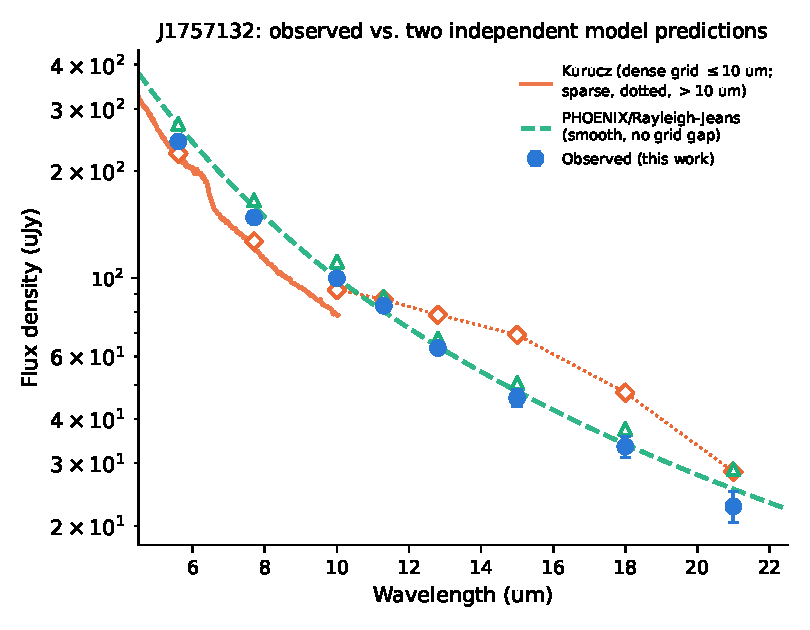
\includegraphics[width=\linewidth]{../figures/j1757132_sed.pdf}
\caption{Observed (blue circles, this work) vs.\ two independent
predictions for J1757132 across all 8 archived MIRI imaging filters:
Kurucz (orange, $T_{\rm eff}=3602$~K, $A_V=0.11$; dotted segment
$>10$~$\mu$m marks a real gap in that grid's own native wavelength
sampling, Section 4) and PHOENIX/Rayleigh--Jeans (aqua, $T_{\rm
eff}=3600$~K; smooth everywhere, no such gap). Per-filter significance
relative to the Kurucz prediction: F560W $+8.0\sigma$, F770W
$+15.6\sigma$, F1000W $+4.9\sigma$, F1130W $-1.1\sigma$, F1280W
$-7.3\sigma$, F1500W $-8.9\sigma$, F1800W $-6.3\sigma$, F2100W
$-2.6\sigma$. The two predictions visibly diverge in shape: the
apparent crossover against Kurucz is largely absent against
PHOENIX/Rayleigh--Jeans, direct visual evidence for Section 4's
conclusion that it is most likely a model-comparison artifact, not a
real spectral feature.
\label{fig:sed}}
\end{figure}

\section{AX-J1600.9-5142}

AX-J1600.9-5142 (F770W: $19.1\sigma$, $T_{\rm eff}=3655$~K,
single-band) is a weaker case, leaning toward a mundane explanation
not yet confirmed. Real, pixel-confirmed diffuse
structure ($\sim13\times$ the photon-noise level) sits in its local
sky background, though a symmetric background model shows this
specific structure does not measurably bias the flux measurement. The
same environment argues for a related, untested mechanism instead: a
cataloged dark nebula and Wolf-Rayet star sit within 1~arcmin
(SIMBAD), and a bright, extended, confusing neighbor sits in WISE's
own beam --- together making PSF-wing leakage the most probable
explanation, though we did not perform the PSF-subtraction/deblending
modeling that would confirm it.

\section{Conclusion and Future Work}

This note reports a validated tool and zero confirmed candidates, not
a completed search. Archive-scale application ($\sim$1000+
stellar-classified MIRI observations) is deferred pending a
candidate-triage strategy beyond simple sigma cuts, and pending two
methodological gaps: validating the Rayleigh--Jeans blackbody
substitute against real cool stars with known mid-IR photometry; and
extending this project's Gaia-based open-cluster membership
cross-match \citep{CantatGaudin2020} to cover currently-uncovered
extragalactic clusters. AX-J1600.9-5142 remains the more promising
target for confirmatory PSF-subtraction follow-up.

\facility{JWST (MIRI)}

\begin{acknowledgments}
This work is based on observations made with the NASA/ESA/CSA JWST,
obtained from MAST. This work presents results from the ESA mission
Gaia, processed by the Gaia Data Processing and Analysis Consortium
(DPAC) and funded by national institutions in the Gaia Multilateral
Agreement; the Two Micron All Sky Survey (University of
Massachusetts/IPAC-Caltech; NASA/NSF); the Wide-field Infrared Survey
Explorer (UCLA/JPL-Caltech; NASA); and the SIMBAD database (CDS,
Strasbourg). The pipeline code is available at
\url{https://github.com/Menrae/jwst-ir-excess}.
\end{acknowledgments}

\software{astropy \citep{Astropy2022}, astroquery, photutils, stpsf, synphot, dust\_extinction, numpy}

\begin{thebibliography}{}

\bibitem[Carrigan(2009)]{Carrigan2009} Carrigan, R.~A. 2009, ApJ, 698, 2075

\bibitem[Griffith et al.(2015)]{Griffith2015} Griffith, R.~L., Wright, J.~T., Maldonado, J., et al. 2015, ApJS, 217, 25

\bibitem[Wright et al.(2014)]{Wright2014} Wright, J.~T., Mullan, B., Sigurdsson, S., \& Povich, M.~S. 2014, ApJ, 792, 26

\bibitem[Libralato et al.(2024)]{Libralato2024} Libralato, M., Argyriou, I., Dicken, D., et al. 2024, PASP, 136, 034502 (also arXiv:2311.12145)

\bibitem[Husser et al.(2013)]{Husser2013} Husser, T.-O., Wende-von Berg, S., Dreizler, S., et al. 2013, A\&A, 553, A6

\bibitem[Castelli \& Kurucz(2003)]{CastelliKurucz2003} Castelli, F., \& Kurucz, R.~L. 2003, in IAU Symposium 210, Modelling of Stellar Atmospheres, ed. N.~Piskunov, W.~W.~Weiss, \& D.~F.~Gray (San Francisco: ASP), A20 (also arXiv:astro-ph/0405087)

\bibitem[Cantat-Gaudin et al.(2020)]{CantatGaudin2020} Cantat-Gaudin, T., Anders, F., Castro-Ginard, A., et al. 2020, A\&A, 640, A1

\bibitem[Lindegren(2018)]{Lindegren2018} Lindegren, L. 2018, Gaia Technical Note GAIA-C3-TN-LU-LL-124

\bibitem[Gordon et al.(2025)]{Gordon2025} Gordon, K.~D., Sloan, G.~C., Garcia Marin, M., et al. 2025, AJ, 169, 6

\bibitem[Astropy Collaboration et al.(2022)]{Astropy2022} Astropy Collaboration, Price-Whelan, A.~M., Lim, P.~L., et al. 2022, ApJ, 935, 167

\end{thebibliography}

\end{document}
